\chapter[Capítulo 4. Diseño del Hardware ]{Diseño del Hardware.}
En la \textbf{ Figura \ref{fig_bloque_c4}} se presenta el diagrama en bloques simplificado del sistema, en dónde el principal corazón es el microprocesador, que será alimentado por la batería del vehículo y se comunicará con el mismo mediante el transceiver CAN.  Los datos obtenidos por el microprocesador serán procesados y enviados a un receptor por medio de un módulo inalámbrico, el receptor desplegará la información en un gráfico entendible para los usuarios del sistema. 
%%%%%%%%%%%%%%%%%%%%%%%%%%%%%%%%%%%%%%%%%%%%%%%%%%%%%%%%%%
\begin{figure}[H]
	\centering
		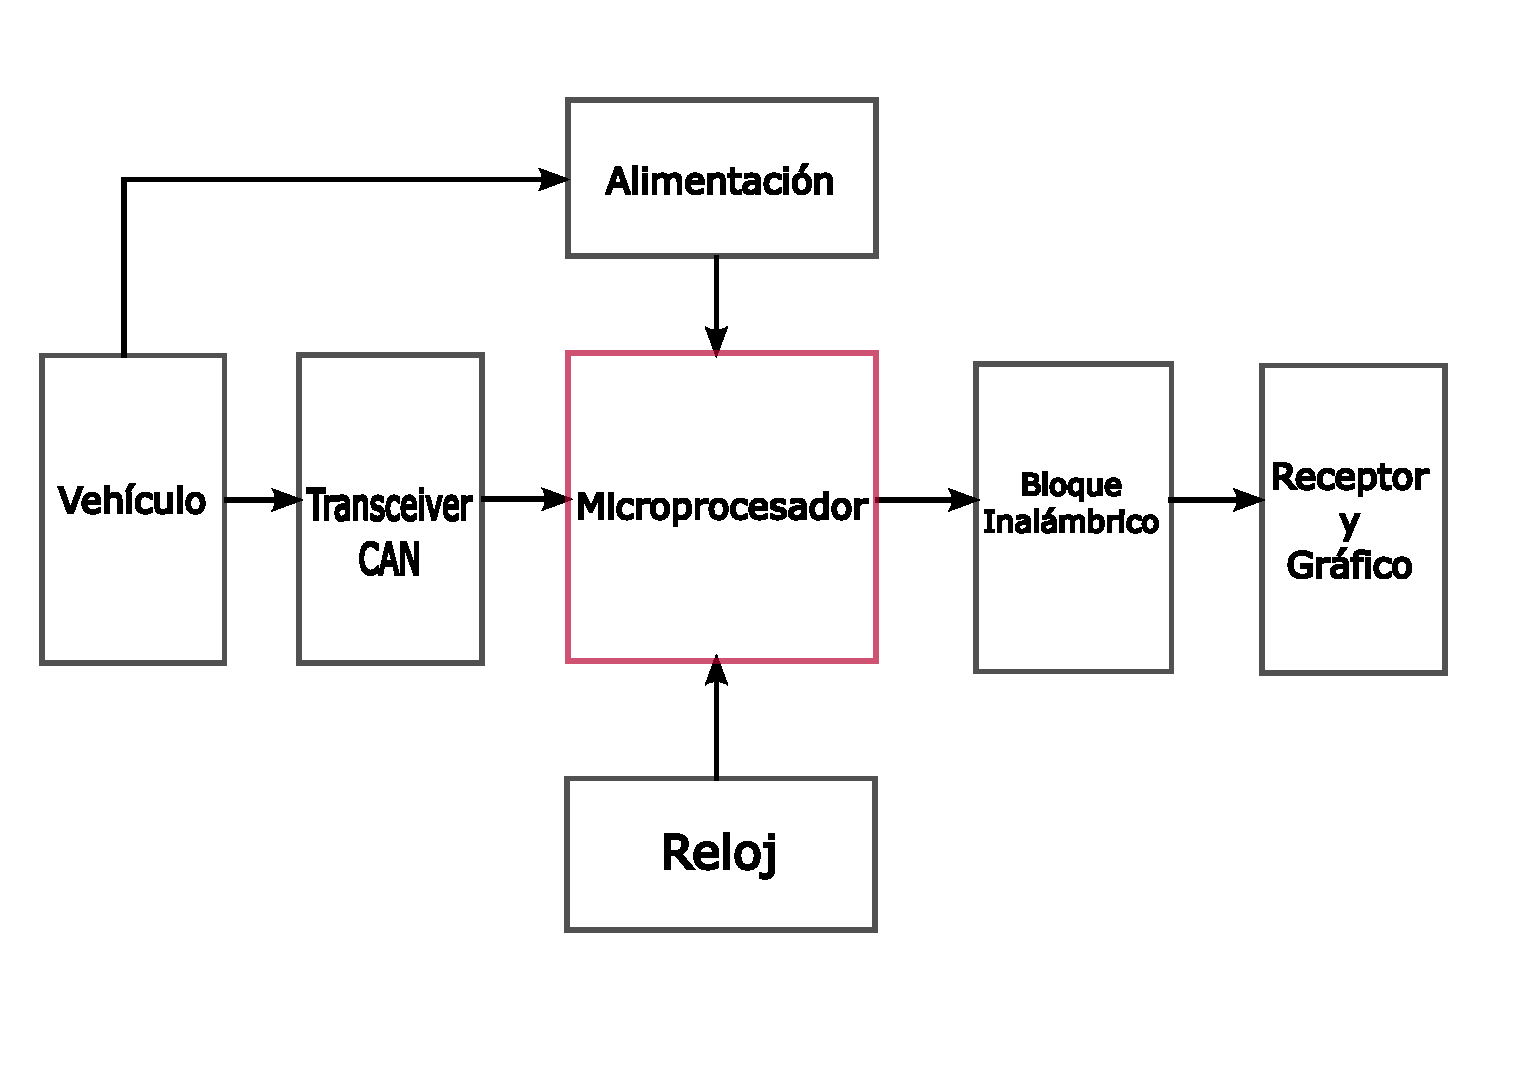
\includegraphics[width=0.9\textwidth]{./Cap4imagen/bloqueHardware.pdf}
	\caption[Diagrama en Bloque del sistema.]{Diagrama en Bloque del sistema.\textbf{ Fuente:}  Elaboración Propia.}
	\label{fig_bloque_c4} % Etiqueta para la referencia.
\end{figure}

% CITAR IMAGEN
%%%%%%%%%%%%%%%%%%%%%%%%%%%%%%%%%%%%%%%%%%%%%%%%%%%%%%%%%%


Para dicho diseño, se utilizará un microcontrolador de la familia PIC (\textit{Peripheral Interface Controller}, por sus siglas en inglés), ya que los PIC son una familia de microcontroladores con amplia documentación técnica y tiene una comunidad de personas activas utilizando estos microcontroladores. Son fabricados por \textit{Microchip Tecnhology Inc.} y existe una gran cantidad de modelos con características y prestaciones, esto nos permite escoger el modelo que se ajusta a la necesidad. Para el Proyecto se utilizó el PIC18F4580 que incluye internamente un módulo CAN y un módulo serial. 
\section{Microcontrolador PIC18F4580}

Las características del módulo CAN incorporado en el PIC son las siguientes:
\begin{itemize}
	\item Aplicación del protocolo CAN 1.2,
	CAN 2.0A y CAN 2.0B.
	\item Tramas de datos estándar y extendidas.
	\item 0-8 bytes de longitud de datos.
	\item Tasa de bits programable hasta 1 Mbit / seg.
	\item Totalmente compatible con módulos CAN PIC18XXX8.
	\item Tres modos de funcionamiento:
	\begin{itemize}
		\item Modo 0: El modo tradicional.
		\item Modo 1: Mejora del modo tradicional con
		apoyo DeviceNet.
		\item Modo 2: Modo FIFO con el apoyo de DeviceNet.
		\end {itemize}
		\item Soporte para tramas remotas con el manejo automatizado.
		\item  Seis memorias intermedias programables como RX y TX, 
		almacenamientos intermedios de mensajes.
		\item 16 filtros de aceptancia.
		\item Dos máscaras de filtro de aceptancia completos que pueden ser asignado a cualquier filtro.
		\item Tres buffers de transmisión dedicados.
		\item Temporizador interno,\cite{DaP}.
		\item Modo de bajo consumo.
	\end{itemize}

Para que el PIC pueda realizar sus funciones es necesario programarlo y hemos de escribir un programa que contenga los procesos que el PIC debe ejecutar para manejar el módulo CAN y operar el protocolo. Este programa se puede escribir en varios lenguajes de programación, pero los  más utilizados son el ’Assembler’ (ensamblador) y el C. En el proyecto se utiliza el lenguaje C por su potencia y robustez para sistemas embebidos, para un último paso y traducir el programa a lenguaje máquina se utiliza el compilador  de CCS (\textit{Custom Computer Services, Inc.}, por sus siglás en inglés).

otras caracterisiticas que se aprovecha del PIC18F4580 son: 
\begin{itemize}
\item {\textbf{Reloj:}} Ofrece varias opciones de configuración de la frecuencia de oscilación, permitiendo al usuario escoger según se adapte a sus necesidades:
Para la elección de la frecuencia de oscilación se ha escogido un clock de 16Mhz.
\item {\textbf{Input/Output:}} En este PIC hay 5 puertos diferentes (A, B, C, D y E). El diseño del hardware utiliza estos puertos para posibles expansiones del circuito o del sistema. 
\item {\textbf{Memoria de programa:}} Tiene 32 kbytes de memoria Flash, suficiente para el diseño del programa.
\item {\textbf{Periféricos:}} En el PIC18F4580 aprovechamos el módulo serial EUSART para comunicar los datos procesador a una central, \cite{DaP}.

\end{itemize}


\subsection{Transceiver BUS CAN MCP2551}
El módulo CAN del  PIC18F4580 precisa de un componente externo llamado transceiver CAN, esto es así para proteger el microcontrolador de cortocircuitos o sobretensiones. Los transceiver están diseñados para uso en aplicaciones de comunicación BUS CAN en la capa física según la norma ISO 11898. El transceiver proporciona una transmisión y recepción de bus diferencial para el controlador CAN y ofrece velocidades de hasta 1Mbps.
El MCP2551 está diseñado para funcionar en ambientes agresivos y cuenta con protección contra sobretensiones, sobrecalentamiento y una amplia gama de modos de servicios. El pin 8 ofrece tres modos de funcionamiento: alta velocidad, control de pendiente, y modos de bajo consumo.
El modo de alta velocidad de funcionamiento se selecciona mediante la conexión del PIN 8 a tierra, permitiendo a los transistores de salida del transmisor encender y apagar lo más rápido posible, el proyecto utiliza este modo de funcionamiento.
Las pendientes de subida y bajada de los bits se pueden ajustar mediante la conexión de una resistencia a tierra en el PIN 8, ya que la pendiente del bit es proporcional a la corriente de salida del PIN. Este control de la pendiente se implementa aplicando valores a la resistencia externa en el PIN 8. Por ejemplo con una resistencia de 10 kohm se logra una pendiente de bit de 15V/us,  y con una resistencia de 100 kohm se logra una pendiente de bit de 2V/us. Si se aplica un nivel lógico alto al PIN 8 el transceiver entra en modo standby, para ahorrar energía y vuelve a su estado de trabajo al aplicar un nivel lógico bajo al PIN 8. El pin Vref 5 está disponible como una referencia de tensión, \cite{sn}.

\subsection{Módulos inalámbricos Xbee}
 los módulos XBee son soluciones integradas que brindan un medio inalámbrico para la interconexión y comunicación entre dispositivos. Estos módulos utilizan el protocolo de red llamado IEEE 802.15.4 para crear redes POINT-TO-MULTIPOINT (punto a multipunto); o para redes PEER-TO-PEER (punto a punto). Fueron diseñados para aplicaciones que requieren de un alto tráfico de datos, baja latencia y una sincronización de comunicación predecible \cite{xbee_c4}, en la \textbf{Figura \ref{fig_xbee_4}} observamos su apariencia. 
 
 %%%%%%%%%%%%%%%%%%%%%%%%%%%%%%%%%%%%%%%%%%%%%%%%%%%%%%%%%%
\begin{figure}[H]
	\centering
		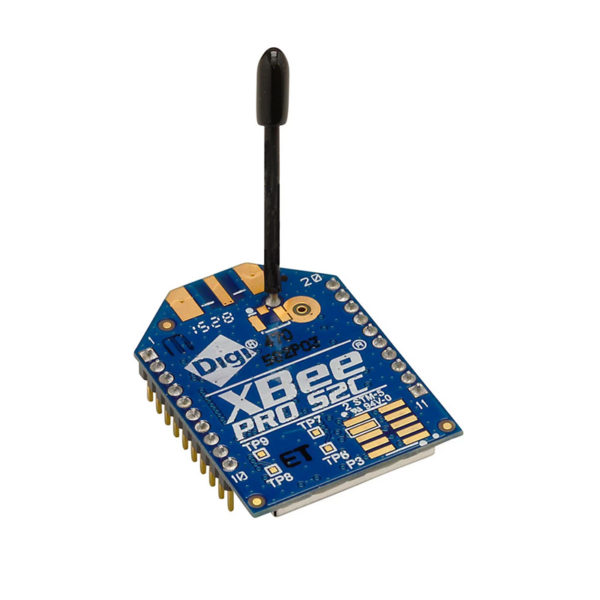
\includegraphics[width=0.6\textwidth]{./Cap4imagen/xbee_modulo.jpg}
	\caption[Fuente de Alimentación.]{Fuente de Alimentación.\textbf{ Fuente:}  \cite{cite_xbee_4}.}
	\label{fig_xbee_4} % Etiqueta para la referencia.
\end{figure}

% CITAR IMAGEN
%%%%%%%%%%%%%%%%%%%%%%%%%%%%%%%%%%%%%%%%%%%%%%%%%%%%%%%%%%

\subsection{Diseño del Hardware}
El montaje implementado es una placa de hardware BUS CAN, basado en el microcontrolador de bajo coste PIC18F4580. La función principal del mismo, es poder leer datos del BUS
CAN y enviarlos a un servidor para mostrarlos en una interfaz gráfica. Para realizar la placa PCB (\textit{Printed Circuit Board}, por sus siglas en inglés) se utilizó el software Proteus, \cite{pro},  el cual es un programa de diseño de diagramas y PCBs con autoenrutador. Proteus tiene una facilidad de uso y configuración.

En la \textbf{Figura \ref{Esch1}} se observa el diagrama del bloque de alimentación del hardware que cuenta con un regulador de tensión LM7805 y dos condensadores electrolíticos cuya función es eliminar el rizado de la señal en la entrada del regulador para que la tensión de salida no tenga variaciones de tensión debido a irregularidades de la fuente principal. 

%%%%%%%%%%%%%%%%%%%%%%%%%%%%%%%%%%%%%%%%%%%%%%%%%%%%%%%%%%
\begin{figure}[H]
	\centering
		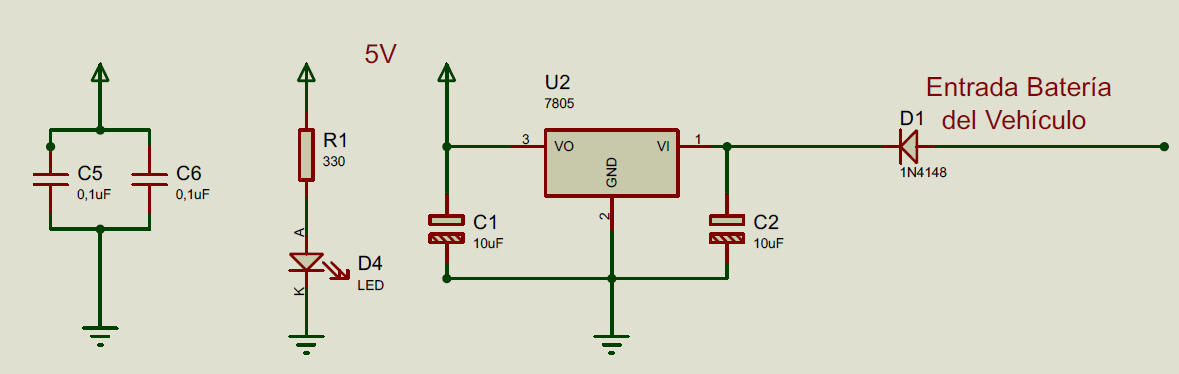
\includegraphics[width=0.6\textwidth]{./Cap4imagen/Fuente5v_4.png}
	\caption[Fuente de Alimentación.]{Fuente de Alimentación.\textbf{ Fuente:} 
	%\cite{sch1}.
	Elaboración Propia.}
	\label{Esch1} % Etiqueta para la referencia.
\end{figure}

% CITAR IMAGEN


%%%%%%%%%%%%%%%%%%%%%%%%%%%%%%%%%%%%%%%%%%%%%%%%%%%%%%%%%%

El Transceiver MCP2551 de Microchips es una interfaz entre el controlador del protocolo BUS CAN que se encuentra en el PIC, y el BUS CAN físico. Este chip está formado por un driver que nos convierte las señales que entran por el CANH  y CANL a señales CMOS para tener una lectura correcta de los datos en el PIC. La configuración de pines no requiere otros elementos aparte de los propios conectores para  entrada, salida y fuente de alimentación. En la \textbf{Figura \ref{Esch2}} se observa la conección donde el PIC será el nodo maestro encargado de escanear y procesar los datos provenientes del bus mediante la ayuda del transceiver CAN. La misma se conectará a un conector OBD II mediante un conector DB9, la alimentación proviene del conector DB9 que ira a extraer la energía de la batería del vehículo.


%%%%%%%%%%%%%%%%%%%%%%%%%%%%%%%%%%%%%%%%%%%%%%%%%%%%%%%%%%%
\begin{figure}[H]
	\centering
		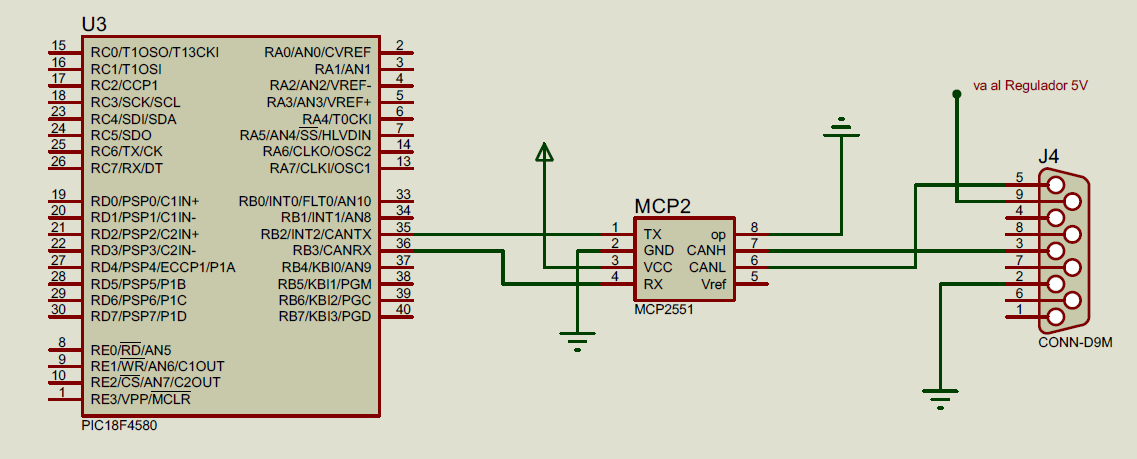
\includegraphics[width=0.6\textwidth]{./Cap4imagen/pic_y_mcp_4.png}
	\caption[Esquemático del Transceiver CAN.]{Esquemático del Transceiver CAN.\textbf{ Fuente:} 
		%\cite{Tu}.
		Elaboración propia}
	\label{Esch2} % Etiqueta para la referencia.
\end{figure}

% CITAR IMAGEN


%%%%%%%%%%%%%%%%%%%%%%%%%%%%%%%%%%%%%%%%%%%%%%%%%%%%%%%%%%%

En la \textbf{Figura \ref{Esch3}} se observa la incorporación de un módulo inalámbrico Xbee para la comunicación con el servidor de datos. 


%%%%%%%%%%%%%%%%%%%%%%%%%%%%%%%%%%%%%%%%%%%%%%%%%%%%%%%%%%%%%
\begin{figure}[H]
	\centering
		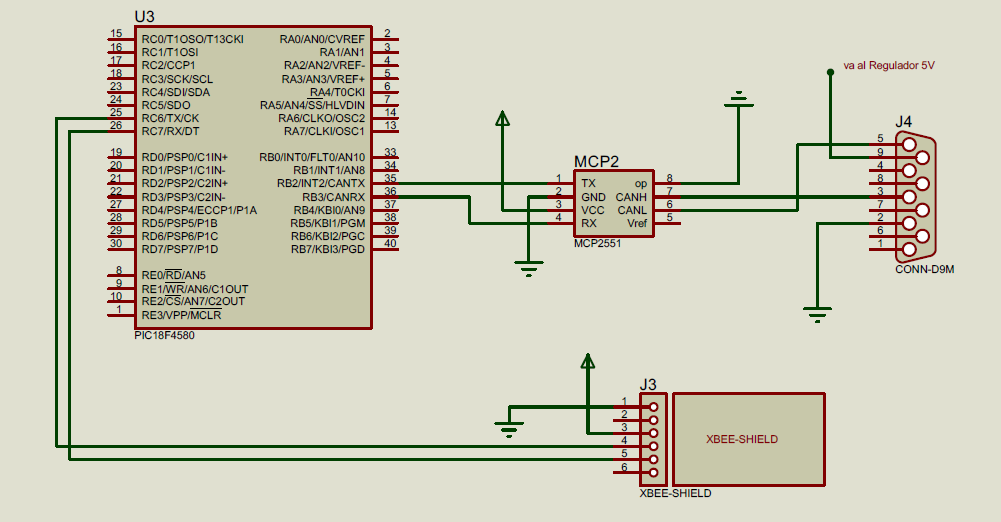
\includegraphics[width=0.6\textwidth]{./Cap4imagen/xbee_4.png}
	\caption[Esquemático PIC y Módulo inalámbrico Xbee.]{Esquemático PIC y Módulo inalámbrico Xbee.\textbf{ Fuente:} Elaboración propia.}
	\label{Esch3} % Etiqueta para la referencia.
\end{figure}

% CITAR IMAGEN


%%%%%%%%%%%%%%%%%%%%%%%%%%%%%%%%%%%%%%%%%%%%%%%%%%%%%%%%%%%%%
 En la \textbf{Figura \ref{Esch5}} que presenta el circuito completo se puede observar los bloques principales del diseño, el Bloque de Programación y Reset, el Bloque de Alimentación y regulación que es alimentado por la batería de 12v del vehículo y luego es reducida a 5v, el Bloque de reloj el cual nos da el clock necesario para configurar la velocidad del bus CAN, el bloque inalámbrico para la comunicación a distancia, el bloque transceiver CAN y el Bloque de entrada del vehículo. 
 

%%%%%%%%%%%%%%%%%%%%%%%%%%%%%%%%%%%%%%%%%%%%%%%%%%%%%%%%%%%%%

%%%Las distancias indicadas son trim = izquierda abajo
%%%derecha arriba, y debe ir siempre seguido del comando clip.
\begin{figure}[H]
	\centering
		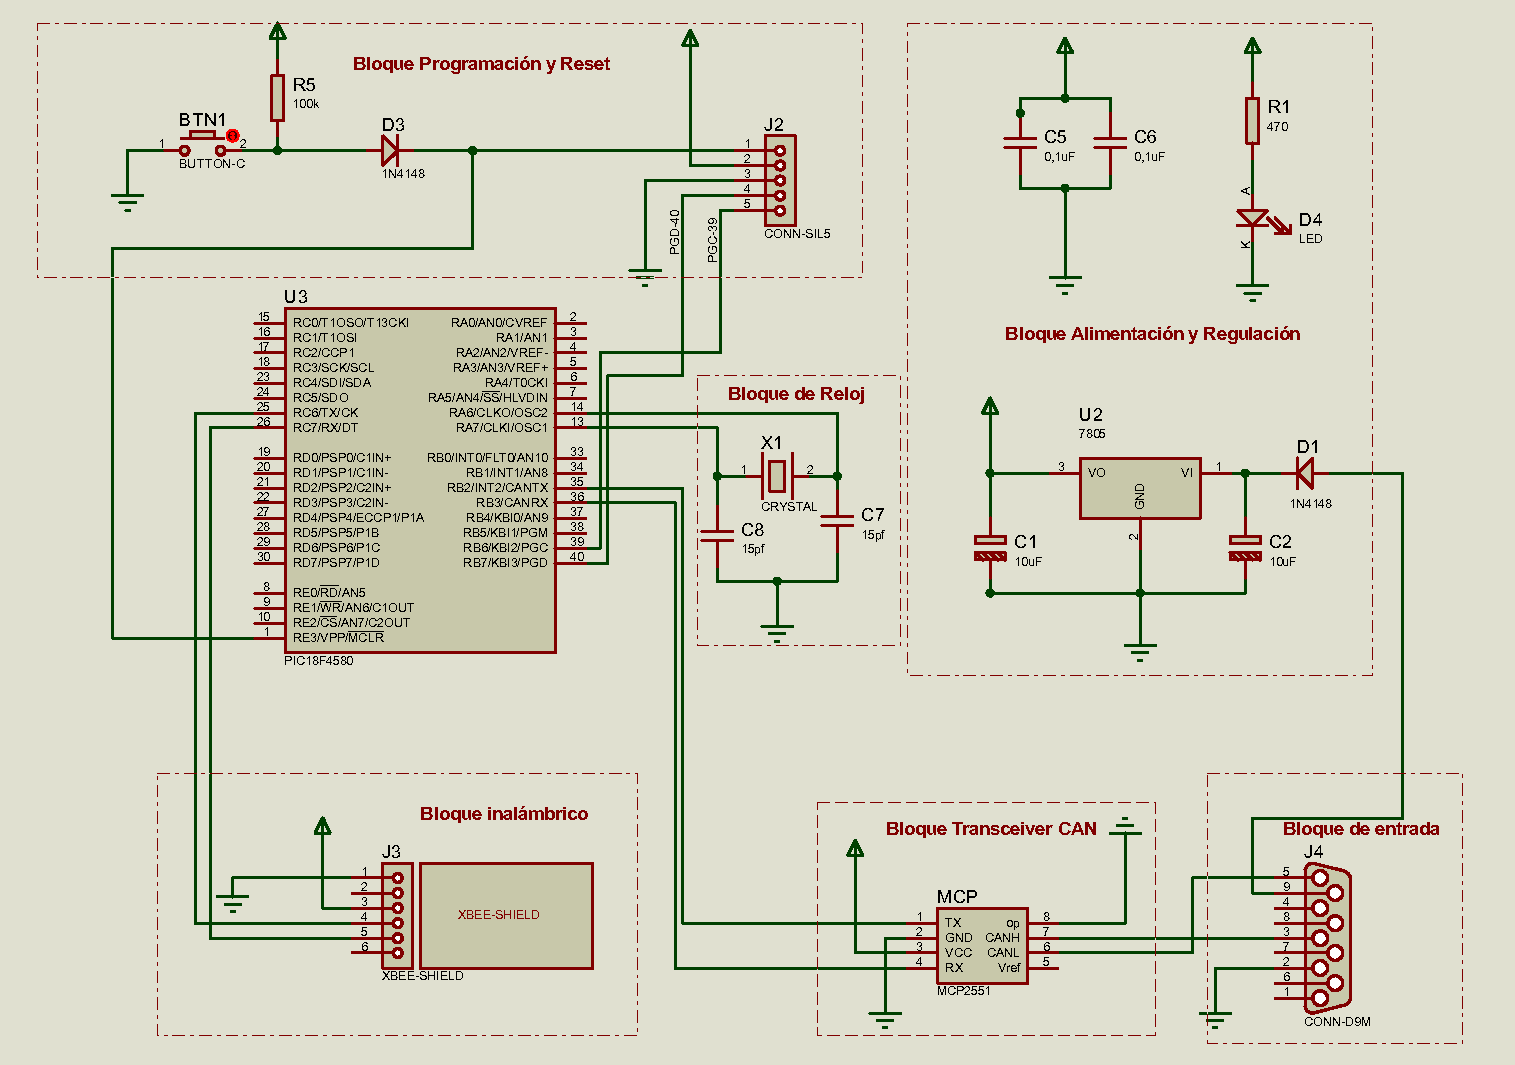
\includegraphics[ width=1\textwidth]{./Cap4imagen/ctocompleto_4.pdf}
	\caption[Diseño del Circuito completo BUS CAN.]{Diseño del Circuito completo BUS CAN.\textbf{ Fuente:} Elaboración propia.}
	\label{Esch5} % Etiqueta para la referencia.
\end{figure}

% CITAR IMAGEN
 En la figura  \textbf{Figura \ref{Esch6}} se puede ver la imagen en PCB y en la que se observa la distribución de los componentes electrónicos en la placa.
%%%%%%%%%%%%%%%%%%%%%%%%%%%%%%%%%%%%%%%%%%%%%%%%%%%%%%%%%%%%%
\begin{figure}[H]
	\centering
		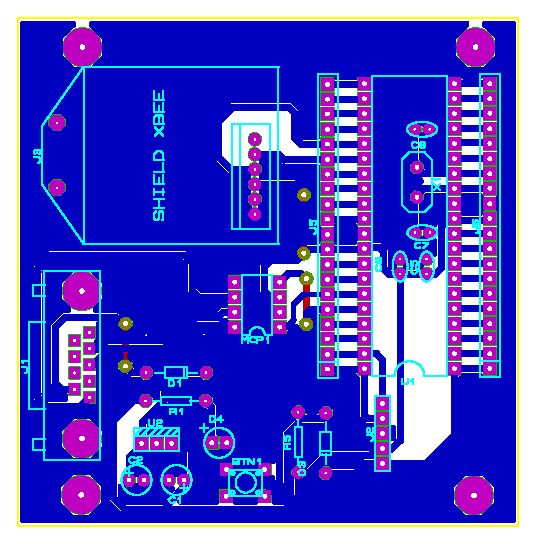
\includegraphics[ width=0.7\textwidth]{./Cap4imagen/pcb_can_4.pdf}
	\caption[ Apariencia del diseño PCB.]{Apariencia del diseño PCB.\textbf{ Fuente:} Elaboración Propia.}
	\label{Esch6} % Etiqueta para la referencia.
\end{figure}

% CITAR IMAGEN


%%%%%%%%%%%%%%%%%%%%%%%%%%%%%%%%%%%%%%%%%%%%%%%%%%%%%%%%%



En la \textbf{Figuras \ref{Esch7} } se muestra las vistas 3D del circuito impreso y ensamblado. 

%%%%%%%%%%%%%    TRANSEIVER         %%%%%%%%%%%%%%%%%%%
\begin{figure}[H]
	\centering
		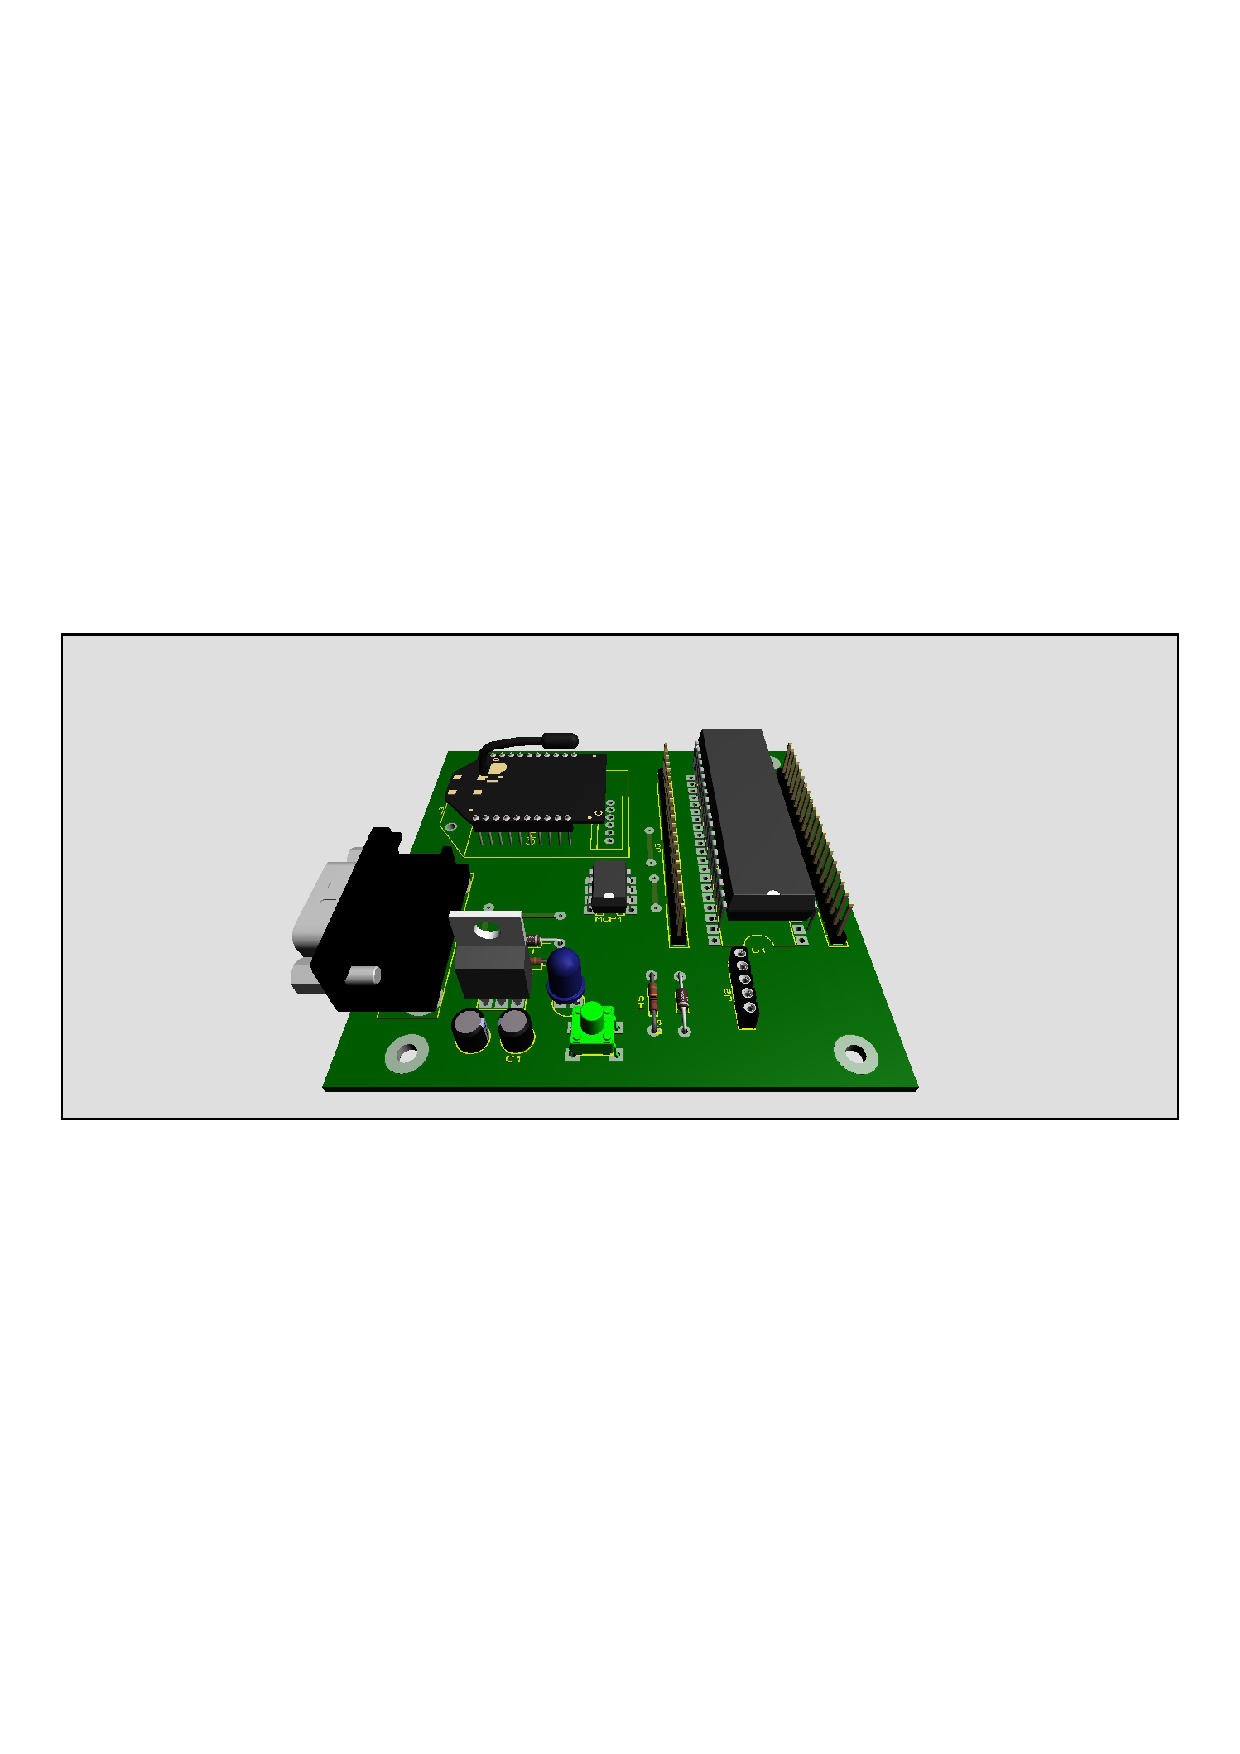
\includegraphics[trim = 10mm 60mm 5mm 50mm, clip, width=0.5\textwidth]{./Cap4imagen/3d_can_4.pdf}
	\caption[Vista 3D del Hardware.]{Vista 3D del Hardware.\textbf{ Fuente:} Elaboración propia.}
	\label{Esch7} % Etiqueta para la referencia.
\end{figure}

% CITAR IMAGEN


%%%%%%%%%%%%%%%%%%%%%%%%%%%%%%%%%%%%%%%%%%%%%%%%%%%%%%%%%%%%%






%%%%%%%%%%%%%%%%%%%%%%%%%%%%%%%%%%%%%%%%%%%%%%%%%%%%%%%%%
\subsection{Proceso de Construcción}
%%%%%%%%%%%%%%%%%%%%%%%%%%%%%%%%%%%%%%%%%%%%%%%%%%%%%%%%

Una vez obtenido el diseño del circuito se procedió a utilizar la máquina CNC (Control Numérico Computarizado)  de la marca Cirqoid para la fabricación del prototipo, este equipo se encuentra en el laboratorio de Sistemas Distribuidos de la FIUNA. La CNC Cirqoid  se encarga de realizar circuitos eléctricos automáticamente  pudiendo realizar los procesos de desgaste de cobre en una PCB, perforado, dispensación de la pasta de soldar y la colocación componentes electrónicos de tipo smd (dispositivos de montaje superficial) , tomando en cuenta que para cada uno de estos procesos tiene su propio cabezal de trabajo, \cite{cirq}. En la \textbf{Figura \ref{Esch8}} se observa la apariencia del sistema y la elaboración de la placa. 


\begin{figure}[H]
	\centering
		\includegraphics[width=0.5\textwidth]{./Cap4imagen/fresado_4.jpg}
	\caption[Proceso de fabricación del circuito PCB con la máquina CNC.]{Proceso de fabricación del circuito PCB con la máquina CNC.\textbf{ Fuente:} Elaboración propia.}
	\label{Esch8} % Etiqueta para la referencia.
\end{figure}

% CITAR IMAGEN


%%%%%%%%%%%%%%%%%%%%%%%%%%%%%%%%%%%%%%%%%%%%%%%%%%%%%%



%###############################################################################
Una vez culminado el proceso en la \textbf{Figura \ref{Esch9}} se presenta la placa pcb terminada. 


\begin{figure}[H]
	\centering
	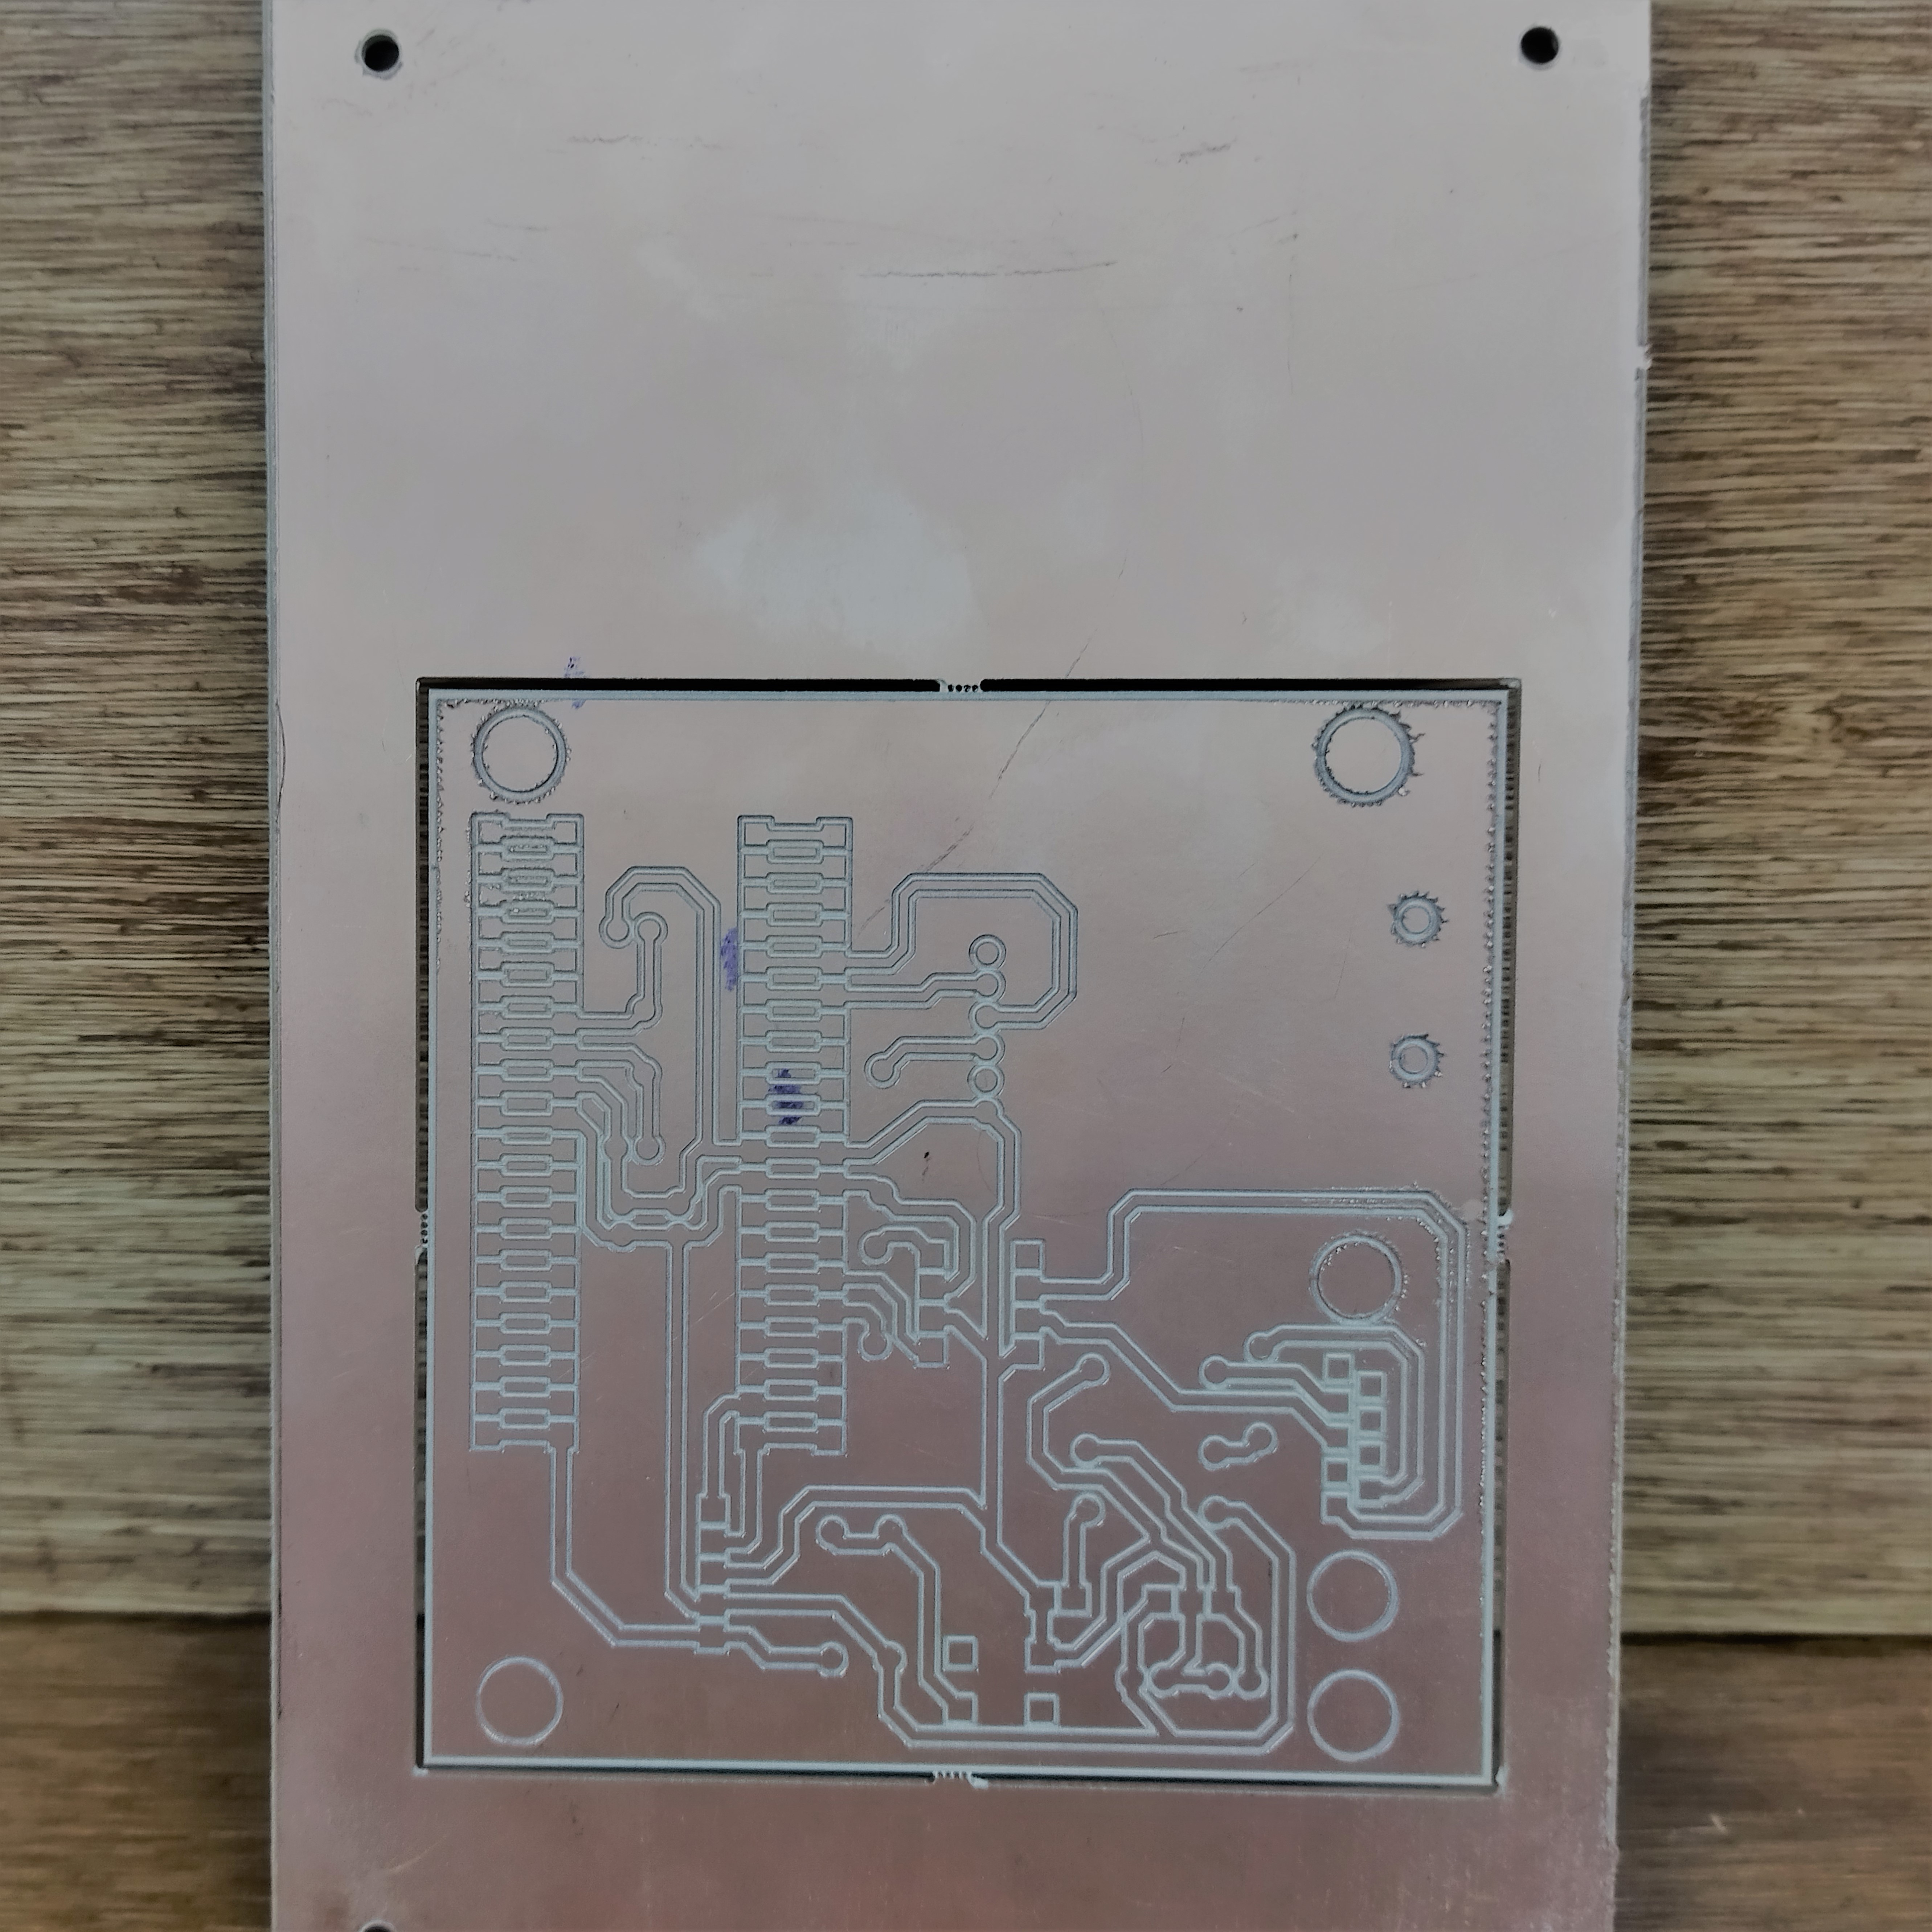
\includegraphics[width=0.5\textwidth]{./Cap4imagen/placa_pcb_4.jpg}
	\caption[Placa impresa.]{Placa impresa. \textbf{ Fuente:} Elaboración propia.}
	\label{Esch9} % Etiqueta para la referencia.
\end{figure}
%###############################################################################


Una vez obtenida el diseño de las pistas del circuito en la placa PCB, se procedió al ensamblado de la misma, resultando el hardware ilustrado en la siguiente \textbf{Figura \ref{Esch10}}.


%###############################################################################
 
\begin{figure}[H]
	\centering
	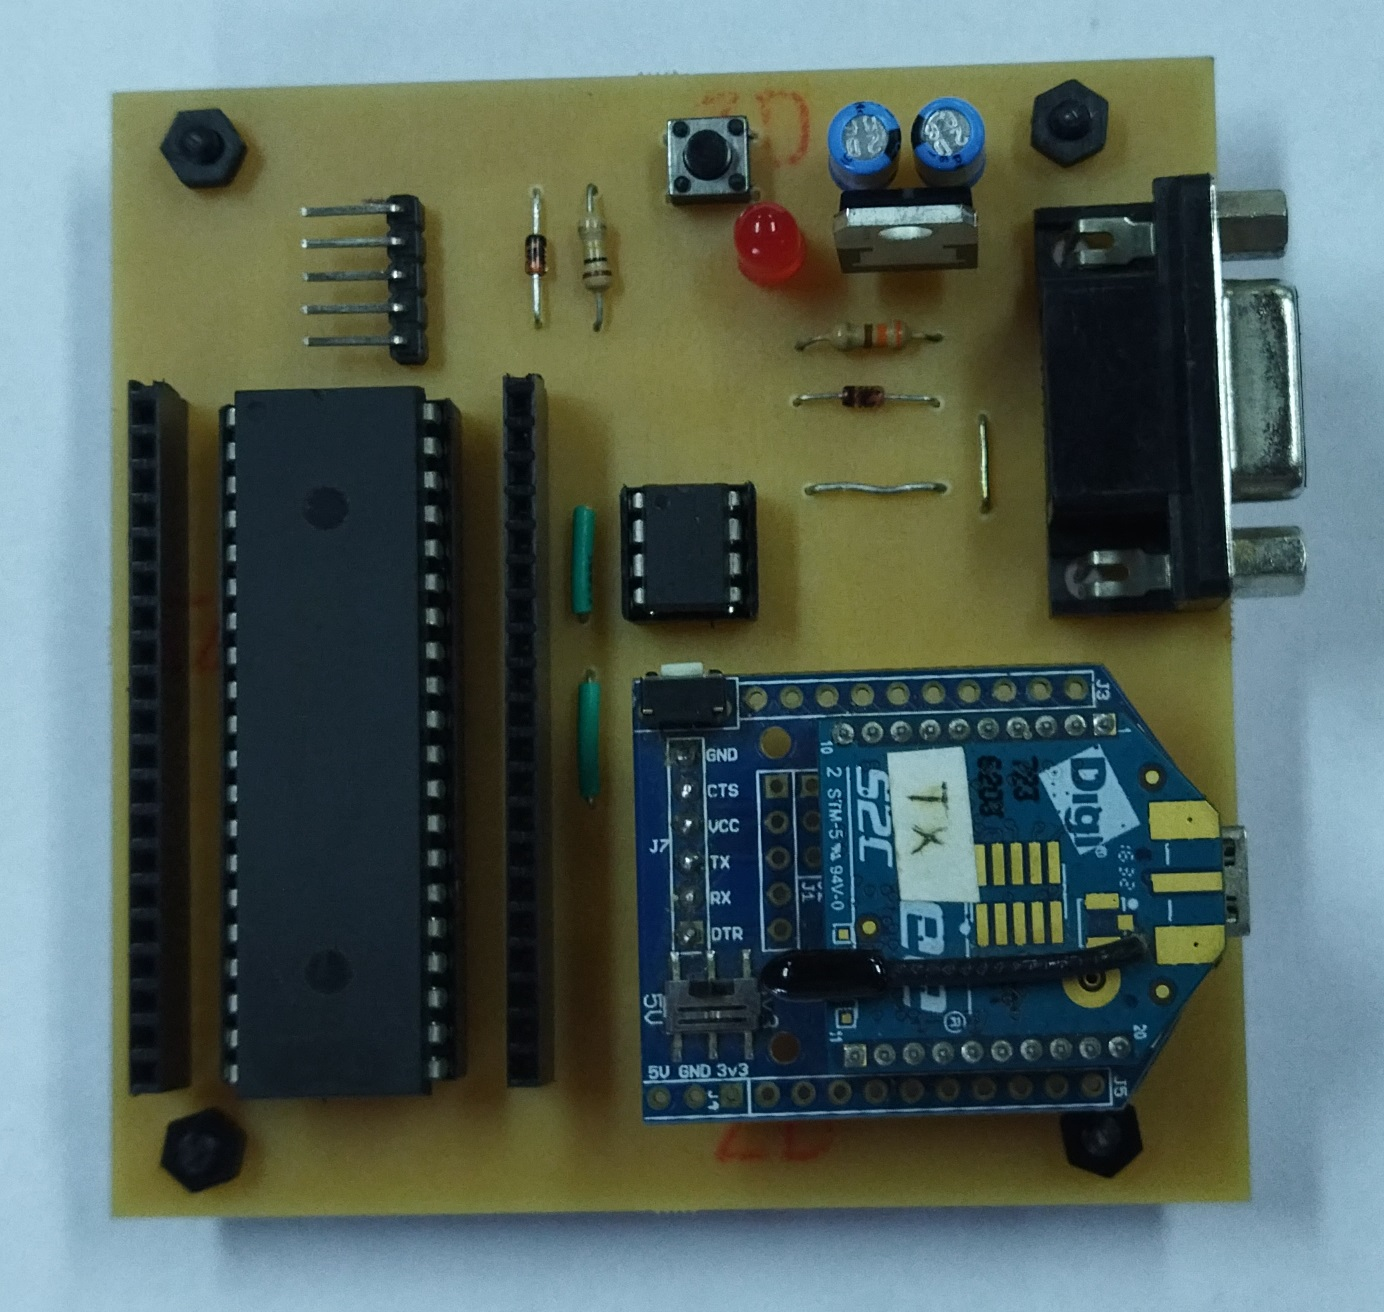
\includegraphics[width=0.5\textwidth]{./Cap4imagen/cto_ensamblado_4.jpg}
	\caption[Vista del Hardware ensamblado.]{Vista del Hardware ensamblado.\textbf{ Fuente:} Elaboración propia.}
	\label{Esch10} % Etiqueta para la referencia.
\end{figure}
%###############################################################################






